%% LaTeX2e class for student theses
%% thesis.tex
%% 
%% Karlsruhe Institute of Technology
%% Institute for Program Structures and Data Organization
%% Chair for Software Design and Quality (SDQ)
%%
%% Dr.-Ing. Erik Burger
%% burger@kit.edu
%%
%% Version 1.3.2, 2017-08-01

%% Available page modes: oneside, twoside
%% Available languages: english, ngerman
%% Available modes: draft, final (see README)
\documentclass[oneside, english]{sdqthesis}

%% ---------------------------------
%% | Information about the thesis  |
%% ---------------------------------

%% Name of the author
\author{Patrick Firnkes}

%% Title (and possibly subtitle) of the thesis
\title{Title of the Thesis\\
Second Title Line}

%% Type of the thesis 
\thesistype{Master's Thesis/Bachelor's Thesis}

%% Change the institute here, ``IPD'' is default
% \myinstitute{Institute for \dots}

%% You can put a logo in the ``logos'' directory and include it here
%% instead of the SDQ logo
% \grouplogo{myfile}
%% Alternatively, you can disable the group logo
% \nogrouplogo

%% The reviewers are the professors that grade your thesis
\reviewerone{Prof. A}
\reviewertwo{Prof. B}

%% The advisors are PhDs or Postdocs
\advisorone{M.Sc. C}
%% The second advisor can be omitted
\advisortwo{M.Sc. D}

%% Please enter the start end end time of your thesis
\editingtime{xx. Month 20XX}{xx. Month 20XX}

\settitle

%% --------------------------------
%% | Settings for word separation |
%% --------------------------------

%% Describe separation hints here.
%% For more details, see 
%% http://en.wikibooks.org/wiki/LaTeX/Text_Formatting#Hyphenation
\hyphenation{
% me-ta-mo-del
}

%% --------------------------------
%% | Bibliography                 |
%% --------------------------------

%% Use biber instead of BibTeX, see README
\usepackage[citestyle=numeric,style=numeric,backend=biber]{biblatex}
\addbibresource{thesis.bib}

%% ====================================
%% ====================================
%% ||                                ||
%% || Beginning of the main document ||
%% ||                                ||
%% ====================================
%% ====================================
\begin{document}

%% Set PDF metadata
\setpdf

%% Set the title
\maketitle

%% The Preamble begins here
\frontmatter

%% LaTeX2e class for student theses: Declaration of independent work
%% sections/declaration.tex
%% 
%% Karlsruhe Institute of Technology
%% Institute for Program Structures and Data Organization
%% Chair for Software Design and Quality (SDQ)
%%
%% Dr.-Ing. Erik Burger
%% burger@kit.edu
%%
%% Version 1.3.2, 2017-08-01

\thispagestyle{empty}
\null\vfill
\noindent\hbox to \textwidth{\hrulefill} 
\iflanguage{english}{I declare that I have developed and written the enclosed
thesis completely by myself, and have not used sources or means without
declaration in the text.}%
{Ich versichere wahrheitsgemäß, die Arbeit
selbstständig angefertigt, alle benutzten Hilfsmittel vollständig und genau
angegeben und alles kenntlich gemacht zu haben, was aus Arbeiten anderer
unverändert oder mit Änderungen entnommen wurde.}
 
 
%% ---------------------------------------------
%% | Replace PLACE and DATE with actual values |
%% ---------------------------------------------
\textbf{PLACE, DATE}
\vspace{1.5cm}
 
\dotfill\hspace*{8.0cm}\\
\hspace*{2cm}(\theauthor) 
\cleardoublepage

\setcounter{page}{1}
\pagenumbering{roman}

%% ----------------
%% |   Abstract   |
%% ----------------
 
%% For theses written in English, an abstract both in English
%% and German is mandatory.
%%
%% For theses written in German, a German abstract is sufficient.
%%
%% The text is included from the following files:
%% - sections/abstract

\includeabstract

%% ------------------------
%% |   Table of Contents  |
%% ------------------------
\tableofcontents

\listoffigures
\listoftables

%% -----------------
%% |   Main part   |
%% -----------------

\mainmatter

%% LaTeX2e class for student theses
%% sections/content.tex
%% 
%% Karlsruhe Institute of Technology
%% Institute for Program Structures and Data Organization
%% Chair for Software Design and Quality (SDQ)
%%
%% Dr.-Ing. Erik Burger
%% burger@kit.edu
%%
%% Version 1.3.2, 2017-08-01

\chapter{Introduction}
\label{ch:Introduction}

%% -------------------
%% | Example content |
%% -------------------

This is the SDQ thesis template.
For more information on the formatting of theses at SDQ, please refer to
\url{https://sdqweb.ipd.kit.edu/wiki/Ausarbeitungshinweise} or to your advisor.

\section{Example: Citation}
\label{sec:Introduction:Citation}
A citation: \cite{becker2008a} For referencing, see \autoref{sec:Introduction:Figures}

\section{Example: Figures}
\label{sec:Introduction:Figures}
\begin{figure}[h]
\centering

\includegraphics[width=4cm]{logos/sdqlogo}
\caption{SDQ logo}
\label{fig:sdqlogo}
\end{figure}

A reference: The SDQ logo is displayed in \autoref{fig:sdqlogo}. 
(Use \code{\textbackslash autoref\{\}} for easy referencing.) 

\section{Example: Tables}
\label{sec:Introduction:Tables}
\begin{table}[h]
\centering
\begin{tabular}{r l}
\toprule
abc & def\\
ghi & jkl\\
\midrule
123 & 456\\
789 & 0AB\\
\bottomrule
\end{tabular}
\caption{A table}
\label{tab:atable}
\end{table}

\section{Example: Todo-Note}
Meaningless text.

\section{Example: Formula}
One of the nice things about the Linux Libertine font is that it comes with
a math mode package.
\begin{displaymath}
f(x)=\Omega(g(x))\ (x\rightarrow\infty)\;\Leftrightarrow\;
\limsup_{x \to \infty} \left|\frac{f(x)}{g(x)}\right|> 0
\end{displaymath}

%% --------------------
%% | /Example content |
%% --------------------
%% LaTeX2e class for student theses
%% sections/content.tex
%% 
%% Karlsruhe Institute of Technology
%% Institute for Program Structures and Data Organization
%% Chair for Software Design and Quality (SDQ)
%%
%% Dr.-Ing. Erik Burger
%% burger@kit.edu
%%
%% Version 1.3.2, 2017-08-01

\chapter{Motivation}
The \textit{Worldwide LHC Computing Grid (WLCG)} is one of the largest grids in the world and processes the data created by the \textit{Large Hadron Collider (LHC)} at CERN \cite{wlcg_update}. 
The created data size steadily increases and reaches 50 Petabytes 2017, thus the grid has to be constantly extended and made more efficient to be able to analyse all data.

However, there is no model or simulation existing to evaluate the load balancing strategies of the grid,
helping the operators to make the correct decisions in the optimization process.

The following chapter describes the WLCG in detail, the current state of the load balancing, and the desired state in the future.

\section{Worldwide LHC Computing Grid}

The WLCG processes 50 Petabytes of data each year created by the LHC at CERN \cite{data_process}
and with its help the \textit{Higgs boson} was discovered in 2012 \cite{wlcg_online}.

170 computing centres distributed in 42 countries are part of the WLCG and it combines 72.000 CPUs, 386 Petabytes online data space and 368 Petabytes nearline space (tape storage) \cite{wlcg_data}. Every day it runs 2 million jobs to analyse data of the CERN experiments.

At CERN there are four experiments, namely: Atlas, Alice, CMS, LHCb. They all use the grid in a similar way, but not entire the same \cite{wlcg_computing}. \Cref{fig:wlcg} shows the hierarchical three tier structure of the WLCG. Tier 0 is the CERN compute centre, which stores all raw data of the experiments, makes the first pass reconstruction and distributes raw data to Tier 1 compute centres. Tier 1 consists of 13 sites, which store a share of raw and reconstructed data, creating a second copy. They also run analysis and simulation jobs. Tier 2 sites, which are mostly located at universities or other scientific institutes, do monte carlo production. In contrast to Tier 1 sites, the Tier 2 sites do not have much storage \cite{wlcg_computing}.

The WLCG is heterogeneous, meaning the resources of one site are different to the resources of another site, the network connections between sites vary, and even the nodes in a single site have different resources. It is trending to use more virtualization, resulting in even more heterogeneity \cite{wlcg_update}.

Our work will focus on modelling and simulating load balancing strategies for the CMS experiment, but because the experiments use the grid in a similar way, the results of our work can be presumably transferred to the other experiments.

	\begin{figure}
		\centering
		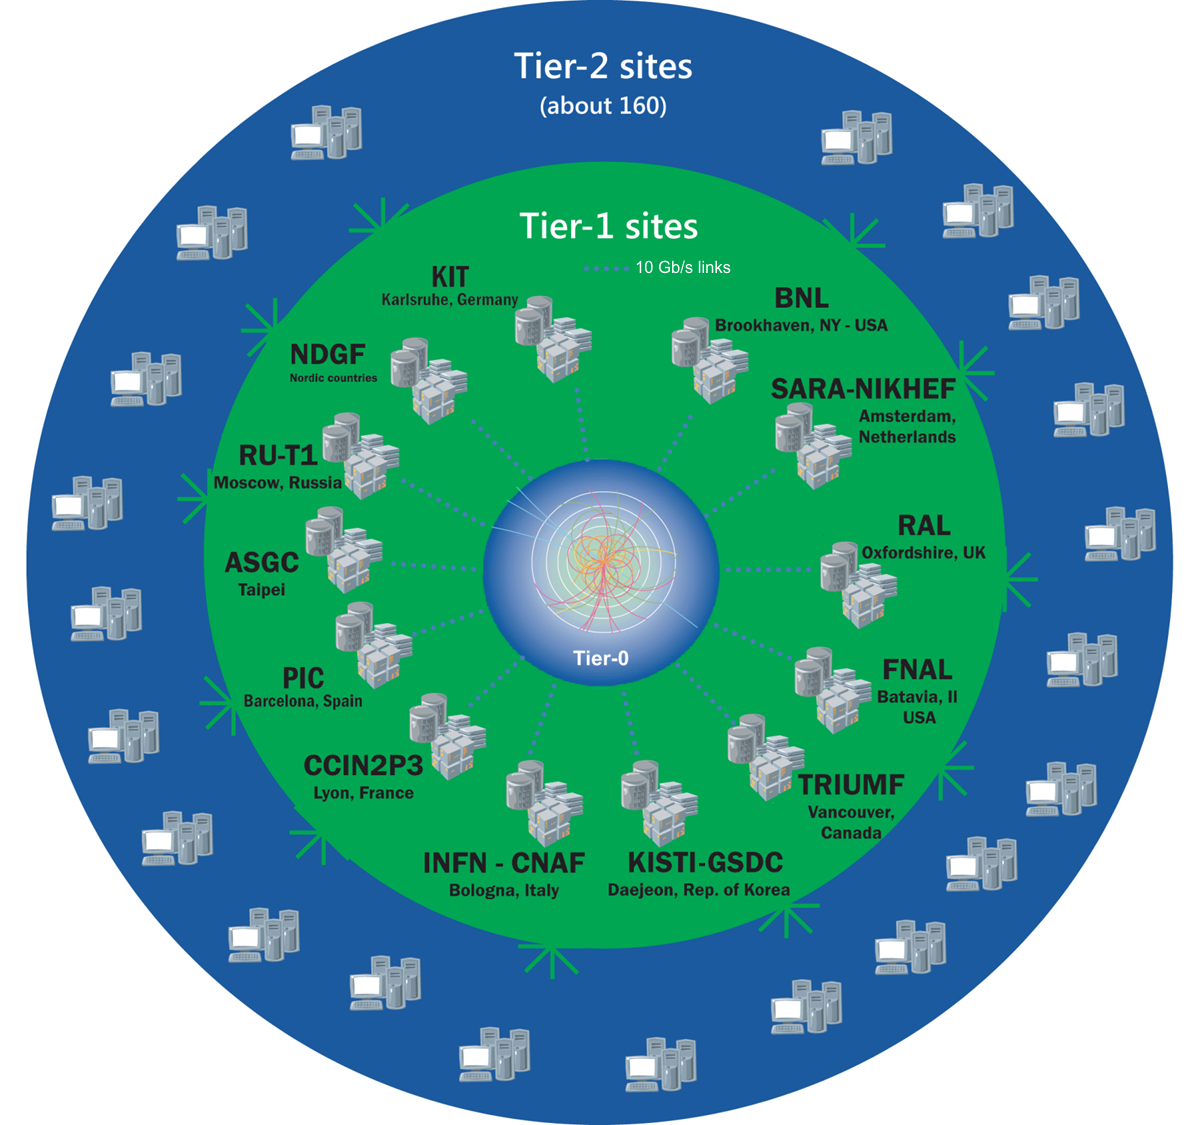
\includegraphics[width=0.65\linewidth]{images/WLCG}
		\caption[]{Tier structure of WLCG \cite{wlcg_tiers}}
		\label{fig:wlcg}
	\end{figure}
	

\section{Current State}
Currently, the load balancing strategy used at the \textit{CMS computing model} is improvable, e.g. it does not account the nature of the jobs: \textit{simulation jobs} require heavy I/O load and \textit{analysis jobs} require heavy CPU time \cite{1742-6596-331-7-072038}. If this nature is not accounted in the scheduling decision, it leads to a bad utilization of the nodes. A good strategy would schedule the right amount of simulation and analysis jobs to a site to maximize the utilisation of I/O and CPU. For example if too many simulation jobs are scheduled, the I/O is creating a bottleneck and the CPUs are idling. 

\textit{HTCondor} is the batch system used at the WLCG and is the central configuration point for the load balancing \cite{wlcg_update}.
It does not only decide on which site a job should run, but even decides on which node, this means it has full control over the load.

There are several other ideas how to improve the CMS computing model beside using a better load balancing strategy, but without a simulation it cannot be evaluated which one is the best in terms of speed-up, cost or utilization.
\newpage

\section{Outlook} TODO 
The amount of data produced by the LHC is steadily increasing, thus either more computing resources have to be provided or the existing ones have to be used in a more efficient way.
However, the computing resources will not increase in the same magnitude as the produced data, hence a better utilization of the given resources is required. Our approach will allow to simulate the effects of different load balancing strategies and decide on these results what the best strategy is. The scheduling problem itself is np complete, so the optimal solution will not be found, but we can decide on a set of strategies which one is the best \cite{1698650}. Evaluating load balancing strategies using the productive system is not accurate, because the workload constantly changes, which makes the performance results of different load balancing strategies incomparable. This problem will be solved by using simulations.

Furthermore, our approach can be used to evaluate the effects of changing the infrastructure of the grid. Therefore, we can find the best approach to improve the CMS computing model, e.g. adding cache, create a new network connection or allow dynamic appearing nodes.
It is difficult to find the best approach without using a simulation, because one cannot consider all side-effects of a change. For example increasing the CPU resources may be a bad decision, because then the network would become the bottleneck and only the increasing of both, the network and the CPU resources would lead to an improvement.

\chapter {Foundations}
In this chapter the \textit{Palladio simulator} is described, which is intended to be used as the tool to model and simulate the load balancing strategies for the CMS computing model.

Another important foundation is to explain the differences between the related concepts of grid and cloud computing in order to classify the CMS computing model.

\section{Palladio}
\label{palladio}
Palladio is a model driven software architecture simulator developed by Karlsruhe Institute of Technology (KIT), FZI Research Center for Information Technology, and University of Paderborn. The development started in 2003 and it is still actively developed today. Palladio predicts quality of software properties (e.g. performance) using several models of a system \cite{BECKER20093}.

These models are the component model, the assembly model, the resource model, the allocation model, and the usage model.
The component model specifies the structure and behaviour of the components independently from their later usage. This allows reuse of the components,  but requires its parametrization.
To represent how the components are connected to model the software architecture the assembly model has to be created. 
The resource model describes the resources environment, including the number and characteristics of the resource containers on which the components could be deployed and the topology of the network connecting these containers.
Allocation models describes how the different components are mapped to the resource containers.
Finally, the usage model describes how a system is used regarding workload, user behaviour, and parameters.

As soon as these models are created, Palladio can be used to simulate the system, choosing one of several supported simulators. \Cref{fig:palladio} shows the whole modelling and simulation process. 

Lehrig and Becker \cite{arch} extended Palladio with the \textit{Architectual Templates} to make it possible to model cloud computing environments efficiently.

Palladio's simulation approach \textit{SimuLizar} was created to simulate self-adaptive systems \cite{becker2013simulizar}.
It was later extended to support the metrics scalability, elasticity, and efficiency \cite{arch}.

The first case studies using Palladio in cloud environments show that the results are accuracy \cite{arch}. However, Palladio was never used to model and simulate such a large system as the CMS computing model.

\begin{figure}
	\centering
	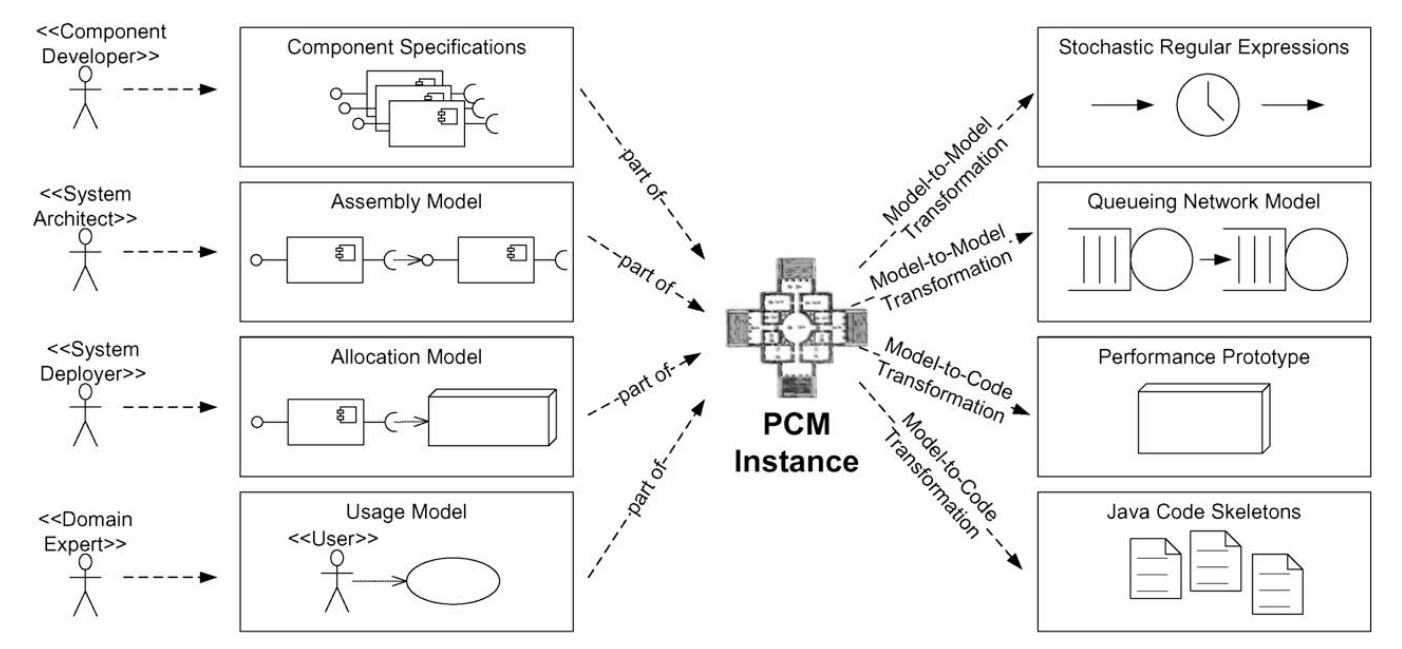
\includegraphics[width=0.95\linewidth]{images/palladio}
	\caption[]{Process of Palladio \cite{BECKER20093}}
	\label{fig:palladio}
\end{figure}



\section{Compare Grid and Cloud Computing}
\label{grid_cloud}
Grid computing is distributed systems working together to solve a problem. 
Cloud computing is a large-scale distributed computing paradigm that is driven by economies of scale.
Both have a lot in common, because cloud computing evolved from grid computing, they are scalable, and involve multi tenancy \cite{foster2008cloud}.
However, there are also some important differences.

Some of the key aspects are: \textit{Resource pooling}, \textit{on-demand resource provisioning}, and \textit{elasticity} \cite{foster2008cloud}.
Firstly, cloud-computing uses massively virtualization, this means that assigning application models to computing nodes do not model the abstraction correctly \cite{cloud_sim}. Instead the resources are pooled and different physical and virtual resources are dynamically assigned and reassigned depending to consumer demand, which makes auto scaling of applications possible \cite{foster2008cloud}.
Secondly, cloud computing allows on-demand resource provisioning \cite{foster2008cloud}. Furthermore, clouds are elastic, they scale up or down according to the currently required resources.

From these aspects it follows, that the CMS computing model is rather a grid than a cloud, because it does not do resource pooling, does not allow on-demand resource provision, and is not elastic.
The given resources are assigned to a job and do not change till its completion, so there is no support of auto scaling \cite{wlcg_update}. The submitted jobs have to wait until resources are free, so there is no on-demand resource provision and it is not elastic, because it does not create new sites if the load is high and does not shut down sites if the load is low \cite{wlcg_update}.


\chapter{State of the Art}
\label{state}
There are a lot of other approaches beside Palladio that deal with the simulation of grids or clouds.
In this chapter a selection of these is presented.


\section{Grid Simulators}
Grid simulators exist since the late 1990s, but the most ones have been created in the mid 2000s. However, most simulators are not developed any more. In this section the most common ones are presented.

\subsection{SimGrid}
\label{simgrid}
\textit{SimGrid} is a framework for simulating large-scale distributed systems and one of the earliest created grid simulators \cite{simgrid_update}. Its first release was 1998 and is one of the few that is still developed today. Originally, it started as a grid simulator, but became more versatile, so that it can be used as a grid, P2P, MPI, or cloud simulator today. Moreover, it is one of the most used grid simulators \cite{simgrid_update}.

In SimGrid the platforms and the deployment are defined in XML, and the application behaviour and scheduling is implemented using C. It supports simulation of CPU, I/O, and network resources, heterogeneous workloads and heterogeneous platforms \cite{simgrid_update}.

It is more scalable than \textit{GridSim}, which is another popular grid simulator \cite{simgrid_update}.
\ref{diag} shows the simulation time of SimGrid and GridSim for 2000 nodes and increasing tasks.
SimGrid performs significantly better that GridSim, because GridSim's simulation time increases quadratic with the number of tasks, while SimGrid's only increases linear. At 500.000 tasks GridSim requires more than one hour and 4.4 GiB of memory to simulate, while SimGrid needs less than 14 seconds and with only 165 MiB of memory.

This performance difference is created by a lot of optimizations, including implementing light-weight execution contexts, using lazy activity updates, and using trace integration for resource management \cite{simgrid_update}.

\begin{center}

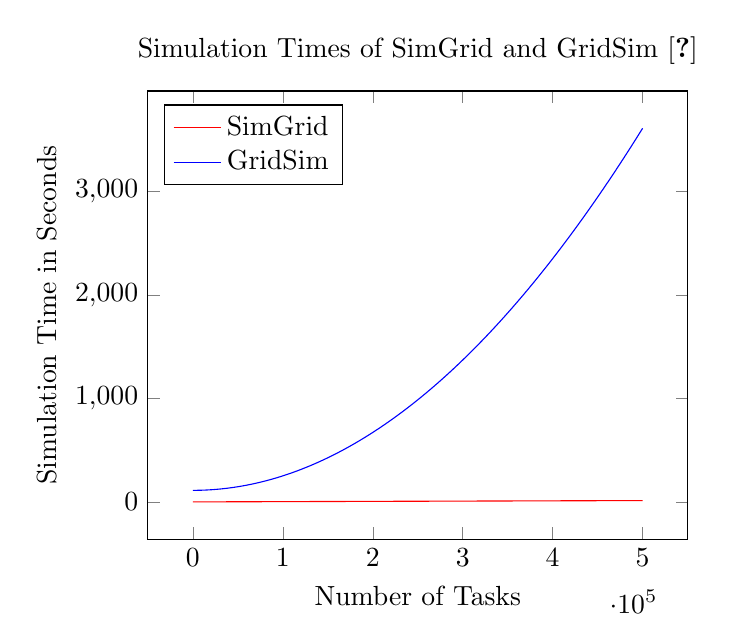
\begin{tikzpicture}
\label{diag}
\begin{axis}[
legend pos=north west,
title=Simulation Times of SimGrid and GridSim \cite{simgrid_update},
xlabel={Number of Tasks},
ylabel={Simulation Time in Seconds},
legend entries={SimGrid, GridSim},]
\addplot [red, domain=1:500000, samples=1000] {0.1*10^(-3)*2000+26*10^(-6)*x};
\addplot [blue, domain=1:500000, samples=1000] {56*10^(-3)*2000+14*10^(-9)*x^2};

\end{axis}
\end{tikzpicture}
\end{center}


\subsection{GridSim}
\label{gridsim}

\textit{GridSim} was created 2001 at the University of Melbourne and was a popular simulator used by other members of the community until its development stopped 2010.
It is focused on evaluating scheduling and resource brokering and supports simulation of CPU, I/O and network resources, heterogeneous workloads and heterogeneous platforms \cite{gridsim}. GridSim is implemented in Java, using SimJava's discrete event simulation \cite{gridsim}.
Sulistio et al. \cite{sulistio2008toolkit} extended GridSim to make more realistic results regarding moving or the storage of data, that the original version struggled with \cite{1698650}. Furthermore, they implemented the simulation of locality of data, to be able to evaluate data replication strategies using GridSim.

However, as in \cref{simgrid} mentioned, GridSim does not scale very well.

\subsection{GangSim}

\textit{GangSim} derived from an enhancement of the \textit{Ganglia Monitoring Toolkit} in 2005 \cite{dumitrescu2005gangsim}, but was not further developed after its initial release.
It is used to handle usage constraints for sites and virtual organizations. It evaluates allocation of individual resources from the interactions between allocation policies across virtual organisations \cite{dumitrescu2005gangsim}.

It supports simulation of CPU, I/O and network resources, heterogeneous workloads and heterogeneous platforms \cite{dumitrescu2005gangsim}.

In difference to most other simulators, it is a discrete time-stepped simulator \cite{dgsim}. This means it will simulate every time slice, even if there is no activity in it. This results in a worse performance and scalability than most discrete event simulators.


\newpage
\subsection{OptorSim}
\textit{OptorSim} was created 2003 as part of the European Data Grid project and is used to evaluate data replication strategies in grids \cite{optorsim}. It simulates the time needed to copy or access the required files for each job and simulates the replication of files according to a given strategy.

It is not developed any more and does not consider job scheduling optimization. Because of its little scope of only evaluating data replication strategies, it does not support the simulation of CPU and I/O resources, or heterogeneous platforms \cite{optorsim}.


\subsection{DGSim}
To improve simulation environments the \textit{DGSim framework} focuses on automating and optimizing the overall simulation process \cite{dgsim}. It helps setting up the experiment by generating realistically grids, grid dynamics and evolution events. Another point is that it either generates realistic grid workloads or uses traces of existing ones. Moreover, it enables grouped or batches of simulations \cite{dgsim}.

It was created in 2007 at Delft University of Technology, and is not public available, thus nobody else beside the authors could use it.


\subsection{ChicagoSim}
Data locality is a important aspect in grid computing, thus \textit{ChicagoSim} was created in 2003 to evaluate different scheduling and data replication algorithms \cite{chicagosim}. In contrast to OptorSim, ChicagoSim not only evaluates data replication algorithms, but also scheduling algorithms. 
One of the insights gained using ChicagoSim is that scheduling jobs to sites containing the data and simultaneously replicating popular data-sets to other sites is a good solution and performs better than scheduling jobs to idle sites and moving the data.

ChicagoSim was not further developed and does not support simulating CPU or I/O resources, instead simple constant waiting times are used, without any concurrence of the underlying resources \cite{chicagosim}. 


\newpage
\section{Cloud Simulators}
In the recent years the research focus migrated from grid to cloud simulators, because grid simulators cannot sufficiently model the cloud infrastructure \cite{compare_grid_cloud}. Although, as in \cref{grid_cloud} shown, the CMS computing model is a grid and therefore a grid simulator is more suitable that an cloud simulator, it is useful to know about the latest developments in cloud simulators. 

Hence, this sections presents a brief overview about the most common cloud simulators.

\subsection{CloudSim}
\textit{CloudSim} was created 2010 at the University of Melbourne as part of the cloudbus project and is the most popular and sophisticated cloud simulator \cite{compare_grid_cloud}. It is based on GridSim and is a foundation for a lot of other cloud simulators.
It shows a good scalability, simulating 100.000 machines in less than 5 minutes, requiring only 75 MB of RAM \cite{survey_clouds}. It supports both system and behaviour modelling of cloud system components such as data centres, virtual machines and resource provisioning policies.

It was later extended with a network simulation component to evaluate applications which communicate with each other \cite{networkcloudsim}.

\subsection{CDOSim}
\textit{CDOSim} was developed 2012 at Kiel University and is a simulator based on CloudSim to evaluate competing cloud deployment options (CDOs) \cite{cdosim}. It represents more the user than the provider perspective and hides fine fine-grained internals of a cloud platform. CDOSim helps to find best ratio between high performance and low costs, by helping to select a cloud provider, the mapping between service and virtual machines, and adoption strategies. 

\subsection{LocalitySim}
Another simulator based on CloudSim is \textit{LocalitySim}, which was created 2016 at the University of Cairo \cite{localitysim}. Data locality affects the performance of any scheduling algorithm. If the scheduler places the job far away from its data, extra time is needed to transfer data. Therefore, LocalitySim was created, because most other cloud simulators are not supporting the locality of data.

\subsection{GreenCloud}
\textit{GreenCloud} focuses on the energy efficiency of clouds \cite{green_cloud}. It was created 2012 
at the University of Luxembourg and focuses specifically on the measurement of energy consumption of severs, switches and links. It simulates the network on a packet level, resulting in a very accurate network model.  

However, it assumes that every server only has a single core and virtualization, storage area networks, and resource management are not considered. Therefore, the correctness of evaluating the trade-off between performance and energy consumption are questionable \cite{survey_clouds}.

\subsection{Cloud Autoscaling Simulation}
Researchers at the Czech Technical University tried to evaluate predictive autoscaler, but found out that CloudSim had accuracy and speed issues \cite{autoscale_cloud}. Thus, they implemented a new simulation method based on \textit{queueing models}, delivering realistic results. 

They found out that autscaling is very stable and cost-efficient when a strategy is used that scales up based on latency and scales down based on utilization. 

\section{MONARC Project}
The \textit{MONARC project} was started 1998 to help with the initial design of the WLCG at CERN \cite{monarc2000models}. They created models and simulations of possible structures of WLCG and developed the MONARC simulator for this purpose. 
The results of the simulations indicated that a hierarchical structure with regional centres performs best, resulting in the 3 Tier structure of the WLCG today \cite{morita2001validation}. 
After its initial results, the MONARC project proposed to model, prototype, and optimise the design of the overall distributed computing and data handling systems for the LHC experiments \cite{monarc2000models}.
However, the project was not continued in 2000.

2004 a second version of the MONARC simulator was released with several improvements, like simulation of data replication. \textit{MONARC2} focuses on simulating experiments at CERN, but can also be used to simulate general large scale distributed computing systems \cite{legrand2003monarc}. A major difference to its first version is, that a discrete-event approach instead of a discrete time-stepped is used, which results in a better performance.

2010 Zach et al. \cite{1742-6596-331-7-072038} used MONARC2 to simulate the ALICE Tier-2 site in Prague. The simulation included 3000 CPUs, and the CPU as well as the network and I/O resources were simulated. MONARC2 delivered accurate simulation results, however two problems occurred. Firstly they were not able to simulate the network load correctly and secondly MONARC2 revealed performance issues, making it not usable for even larger systems.

\section{CACTOS}
\textit{CACTOS} is an approach to cloud infrastructure automation and optimization, started in 2014 as project funded by the European Union \cite{cactos}.
One part of the approach is the \textit{CACTOS Runtime Toolkit} for monitoring and resource management and an other part is the \textit{CACTOS Prediction Toolkit} for evaluation of alternative data centre deployment scenarios and resource management algorithms.

The Prediction Toolkit is built on Palladio and SimuLizar, see \cref{palladio} for details on Palladio.
The models used by the Prediction Toolkit regarding resources or application behaviour are updated using monitoring data to handle the highly dynamic behaviour of clouds.
The idea to couple monitoring and grid simulation tools has been around for a while, suggested by Pop et al. \cite{1698650} in 2006.

CACTOS supports the rapid testing of resource management algorithms due the ability to simulate them without reimplementing the algorithms for the Prediction Toolkit and automatic creation of workload models by using runtime monitoring data \cite{rapidtesting}. Most other simulators require the reimplementation of a resource management algorithm to its specific interface.

First case studies show that the Prediction Toolkit has a high accuracy, but it was not tested on large systems yet \cite{rapidtesting}.

\chapter{Discussion}
\label{dis}
Several grid and cloud simulators have been presented in \cref{state}. Grid simulators suit our needs better for modelling and simulating the CMS computing model, see \cref{grid_cloud} for the differences of grid and cloud computing. It may be possible to use a cloud simulator, but the additional functionalities to simulate clouds may create an overhead, affecting performance and comprehensibility of the simulation due to the required workarounds. Nevertheless, it seems that CloudSim is the most evolved cloud simulator.

\Cref{compare} compares the presented grid simulators based on our needs. As one can see only SimGrid and Palladio do fulfil them, but for Palladio its not clear if its as scalable as required. Though, as part of the CACTOS project Palladio and SimuLizar are made ready for the cloud, so we expect that it will fulfil our scalability needs. All other simulators are either not developed any more or have never been intended to be used as a general grid simulator, instead they only have been created for the research of a small scope in grid computing. Most simulators support the simulation of CPU, I/O, and network resources. Also heterogeneous platforms and tasks are mostly supported.

As mentioned in \cref{state} GridSim, OptorSim, ChicagoSim and LocalitySim are the only simulators that consider data locality. However, this feature is not required for simulating load balancing strategies, because we only need to simulate the effects of a data replication strategy, e.g. reduce the data miss rate by 30\%. The data locality feature is needed to evaluate better data replication strategies. 

There was no indication that a similar large grid or cloud as the CMS computing grid was simulated yet, so our work will evaluate if the existing tools make it possible to simulate such large systems.


\begin{center}
\label{compare}
\captionof{table}{Comparison of Grid Simulators} 
\scalebox{0.8}{
\begin{tabular}{|c|c|c|c|c|c|c|c|c|c|}
	\hline
	\rot{Simulator} & \rot{Active Project} & \rot{General usable} & \rot{Job Scheduling} & \rot{CPU} & \rot{I/O} & \rot{Network} & \rot{Heterogeneous Platforms  } & \rot{Heterogeneous Tasks} & \rot{Scalable} \\
	\hline
	SimGrid & \cmark&\cmark&\cmark&\cmark&\cmark&\cmark&\cmark&\cmark&\cmark\\
	\hline
	GridSim & \xmark&\cmark&\cmark&\cmark&\cmark&\cmark&\cmark&\cmark&\xmark\\	
	\hline
	GangSim & \xmark&\xmark&\cmark&\cmark&\cmark&\cmark&\cmark&\cmark&\xmark\\	
	\hline
	OptorSim & \xmark&\xmark&\xmark&\xmark&\xmark&\cmark&\xmark&\cmark&\qmark\\	
	\hline
	DGSim & \xmark&\xmark&\cmark&\xmark&\cmark&\cmark&\cmark&\cmark&\cmark\\	
	\hline
	ChicagoSim & \xmark&\xmark&\cmark&\xmark&\xmark&\cmark&\cmark&\cmark&\cmark\\	
	\hline
	MONARC & \xmark&\cmark&\cmark&\cmark&\cmark&\cmark&\cmark&\cmark&\xmark\\	
	\hline
	Palladio & \cmark&\cmark&\cmark&\cmark&\cmark&\cmark&\cmark&\cmark&\qmark\\	
	\hline

\end{tabular}
}
\end{center}

\chapter{Conclusion}

It was shown that Palladio is a decent choice to use for modelling and simulation of the load balancing strategies of the CMS experiment. Another good candidate is SimGrid. However, if it shows up that Palladio is not scalable enough, model-to-model TODO transformations can be used to transform Palladio models to SimGrid models and use SimGrid to simulate the load balancing strategies. Also, we keep CloudSim in mind, because it is the most sophisticated cloud simulator.

Another insight gained is that the need for a simulation to optimize the WLCG was already around in the early 2000s. Nevertheless, the MONARC project did not continue its work, so no simulation is existing yet. 

Furthermore, it was shown that neither the CMS computing experiment nor any other similar large grid or cloud system was simulated yet. Our work will create a model and a simulation magnitudes larger than the existing ones and will show if the simulators of today can be used to accurately model such large systems.

\chapter{Outlook}
The first step will be to use Palladio to model and simulate the Tier 1 centre \textit{GridKA} of the CMS computing model. 
To achieve that, performance logs have to be analysed to find out the different types of executed jobs, 
their frequency and resources requirements. Also, the resources of GridKA have to be determined.
After the model is created and calibrated with the measured performance values, the simulation can be executed and the results can be validated.
At this point load balancing strategies of a single site could be simulated, adapting the workload of the site according to the expected effects of changing the global load balancing strategy.

The model of GridKA is then used as the foundation to model the whole CMS computing model. Finally, the load balancing of the whole CMS computing model can be simulated, which allows the simulation of all side effects between the sites.

%% LaTeX2e class for student theses
%% sections/evaluation.tex
%% 
%% Karlsruhe Institute of Technology
%% Institute for Program Structures and Data Organization
%% Chair for Software Design and Quality (SDQ)
%%
%% Dr.-Ing. Erik Burger
%% burger@kit.edu
%%
%% Version 1.3.2, 2017-08-01

\chapter{Evaluation}
\label{ch:Evaluation}

%% -------------------
%% | Example content |
%% -------------------
\dots

\section{First Section}
\label{sec:Evaluation:FirstSection}

\dots

\section{Second Section}
\label{sec:Evaluation:SecondSection}

\dots

\section{Third Section}
\label{sec:Evaluation:ThirdSection}

\dots
%% ---------------------
%% | / Example content |
%% ---------------------
%% LaTeX2e class for student theses
%% sections/conclusion.tex
%% 
%% Karlsruhe Institute of Technology
%% Institute for Program Structures and Data Organization
%% Chair for Software Design and Quality (SDQ)
%%
%% Dr.-Ing. Erik Burger
%% burger@kit.edu
%%
%% Version 1.3.2, 2017-08-01

\chapter{Conclusion}
\label{ch:Conclusion}

\dots

%% --------------------
%% |   Bibliography   |
%% --------------------

%% Add entry to the table of contents for the bibliography
\printbibliography[heading=bibintoc]

%% ----------------
%% |   Appendix   |
%% ----------------
\appendix
%% LaTeX2e class for student theses
%% sections/apendix.tex
%% 
%% Karlsruhe Institute of Technology
%% Institute for Program Structures and Data Organization
%% Chair for Software Design and Quality (SDQ)
%%
%% Dr.-Ing. Erik Burger
%% burger@kit.edu
%%
%% Version 1.3.2, 2017-08-01


\iflanguage{english}
{\chapter{Appendix}}    % english style
{\chapter{Anhang}}      % german style
\label{chap:appendix}


%% -------------------
%% | Example content |
%% -------------------
\section{First Appendix Section}
\label{sec:appendix:FirstSection}
		
\setcounter{figure}{0}
		
\begin{figure} [ht]
  \centering
  \caption{A figure}
  \label{fig:anotherfigure}
\end{figure}


\dots
%% ---------------------
%% | / Example content |
%% ---------------------

\end{document}